\documentclass[a4paper,11pt]{article}
\usepackage[utf8]{inputenc}
\usepackage[russian]{babel}
\usepackage[T1]{fontenc}
\usepackage{amssymb,amsmath,graphicx,indentfirst}
\usepackage{caption}
\usepackage{clrscode}
\usepackage[unicode]{hyperref}

\setlength{\parskip}{1ex plus 0.5ex minus 0.2ex}

\author{Олег Смирнов\\
\texttt{oleg.smirnov@gmail.com}}
\date{27 октября 2011 г.}
\title{Построение и анализ алгоритмов -- Лекция 5. Сортировка за линейное время
\\(конспект Ивана Веселова)}

\begin{document}

\maketitle
\tableofcontents
\newpage

\setlength{\parskip}{1ex plus 0.5ex minus 0.2ex}

\section*{Цель лекции}
\begin{itemize}
\item Нижняя граница сортировки сравнением
\item Деревья решений
\item Сортировка подсчётом
\item Поразрядная сортировка
\end{itemize}

\section{Насколько быстро мы можем сортировать?}
Это зависит от \emph{модели вычислений} -- то есть того, что нам разрешено
делать с элементами.

Все алгоритмы сортировки, что мы успели изучить являются примерами сортировки
сравнениями, т.е. мы можем использовать сравнения чтобы определить относительный
порядок элементов. Лучшим результатом, который нам пока удалось достичь является
$O(n \log n)$. Можно ли достичь лучшего результата? Нам помогут разобраться в
этом \emph{деревья решений}.

\section{Деревья решений}

Предположим, что нам нужно решить задачу сортировки трёх чисел.

Запишем алгоритм не в обычной текстовой форме, а в виде дерева. Для того, чтобы
определить порядок элементов мы сравниваем их. Внутренние узлы дерева,
помеченные как $i:j$ представляют собой сравнение двух элементов: $a_i, a_j$.
\begin{itemize}
\item если $a_i \leqslant a_j$, то мы идём по левой ветке
\item если $a_i > a_j$. то по правой
\end{itemize}

В листьях дерева находятся перестановки $\langle \pi(1), \pi(2), \ldots \pi(n)
\rangle $, такие что $a_{\pi(1)} \leqslant a_{\pi(2)} \leqslant \ldots \leqslant a_{\pi(n)}$

Рассмотрим пример, когда массив состоит из чисел 9, 4 и 6:

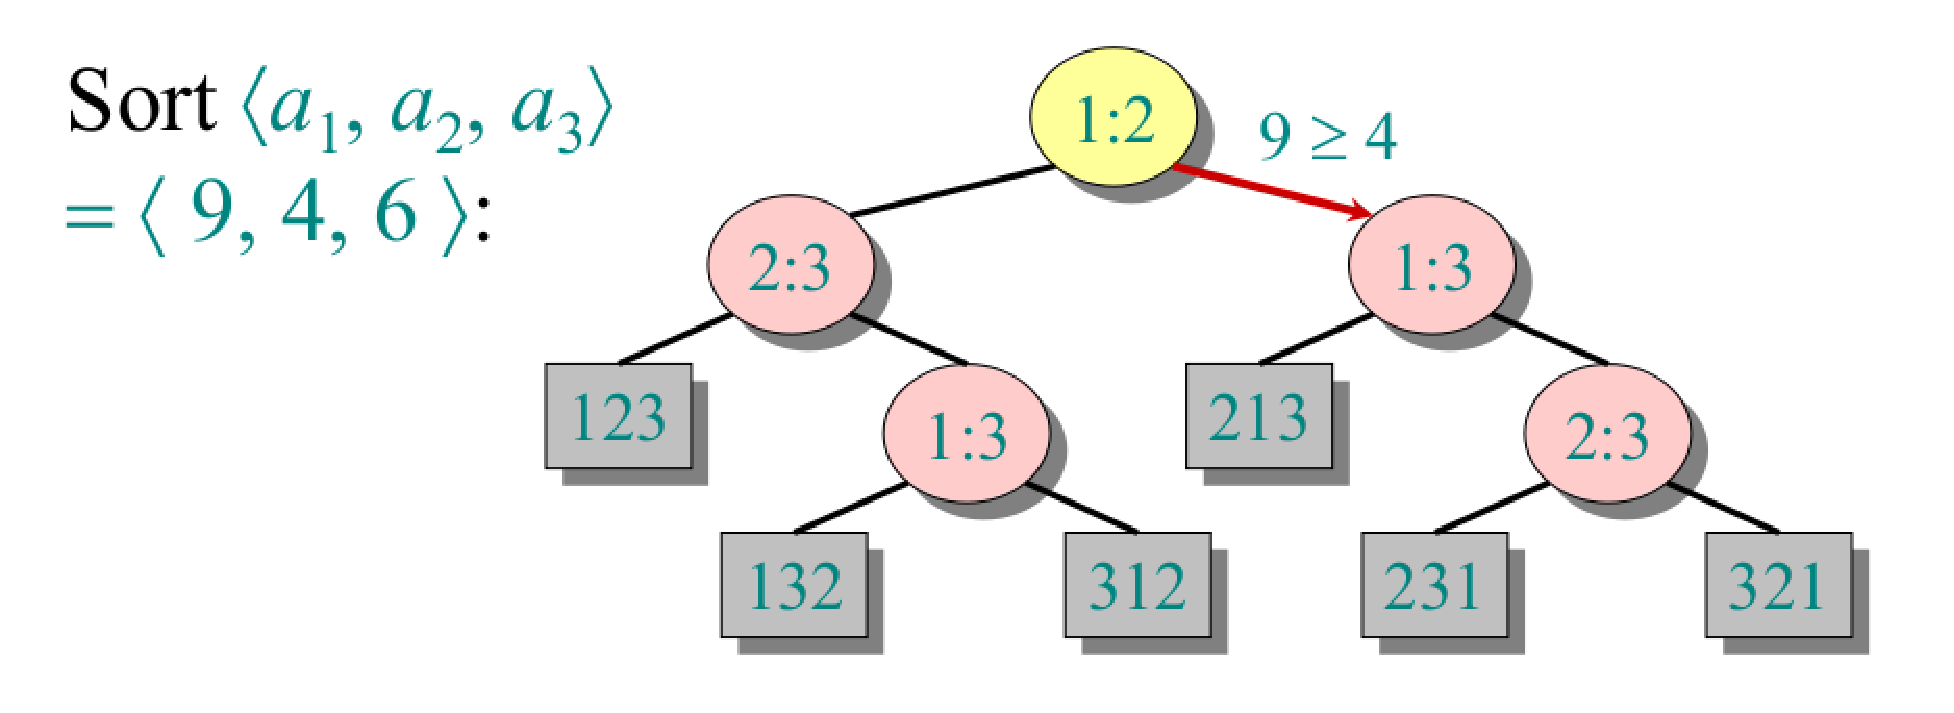
\includegraphics[width=5in]{lecture5/tree2.eps}

Деревом решений можно смоделировать любой алгоритм сортировки сравнениями:
\begin{itemize}
\item одно дерево для каждого размера входных данных -- $n$
\item можно рассматривать алгоритмы как набор сравнений, причём каждое сравнение
  -- это очередное ветвление дерева
\item дерево содержит все возможные варианты выполнения алгоритма
\item время выполнения алгоритма = длина выбранного пути от корня до листа с
  финальной перестановкой-решением
\item наихудшее время выполнения = высота дерева
\end{itemize}

С помощью этой модели можжно доказать следующую теорему: любое дерево решений,
сортирующее $n$ элементов имеет высоту $\Omega(n \lg n)$.

Доказательство: обозначим количество листьев дерева как $l$. Поскольку дерево
должно уметь сортировать все возможные варианты входных данных в нём должно быть
как минимум $n!$ листьев, отсюда неравенство $l \geqslant n!$. Тем не менее
поскольку дерево бинарное, количество его листьев ограничивается $2^h$, где $h$
-- высота дерева, т.е. $l \leqslant 2^h$. Из этих двух неравенств получаем
третье: $2^h \geqslant n!$

Поскольку логарифм -- монотонно возрастающая функция, то:

$$h \geqslant \lg n! \geqslant \text{(по формуле Стирлинга)} \geqslant \lg (n/e)^n
= n \lg(n/e) = n\lg n - n \lg e = \Omega(n \lg n)$$

Таким образом, можно сделать вывод, что сортировка слиянием является
асимптотически оптимальной.

\section{Сортировка подсчётом}

Эта сортировка применима в том случае, если нужно отсортировать целые числа в
заданном (не очень большом) диапазоне.

Вход: массив $A[1 \ldots n]$, где $n \in \lbrace 1, 2, \ldots, k \rbrace$

Результат: остортированный массив $B[1 \ldots n]$

Вспомогательный массив: $C[1 \ldots k]$

Идея состоит в подсчёте количества элементов, меньших чем заданный и последующем
выборе места для элемента на основе этих данных. Например если известно, что 15
элементов меньше рассматриваемого элемента, то очевидно, что его место в
отсортированном массиве будет равно 16. Однако в массиве может быть несколько
одинаковых элементов, потому необходимо несколько модифицировать алгоритм.

\begin{codebox}
\li \For $i \gets 1 $ \To $k$
\li      \Do $C[i]] \gets 0$ \End
   
\li \For $j \gets 1 $ \To $n$
\li      \Do $C[A[j]] \gets C[A[j]] + 1$ \End
 
\li \For $i \gets 2 $ \To $k$
\li      \Do $C[i] \gets C[i] + C[i-1]$ \End

\li \For $j \gets n $ \Downto $1$
\li      \Do $B[C[A[j]]] \gets A[j]$
\li          $C[A[j]] \gets C[A[j]] - 1$
         \End
\end{codebox}

В первом цикле обнуляется массив-счётчик, во втором цикле определяется
количество вхождений каждого элемента. В третьем берутся префиксные суммы, то
есть определяется количество элементов меньших или равных заданному. В четвёртом
цикле происходит расстановка элементов по местам согласно значению массива-счётчика.

Пример (на лекции лучше рассмотреть пример покороче: 4 1 3 4 3):

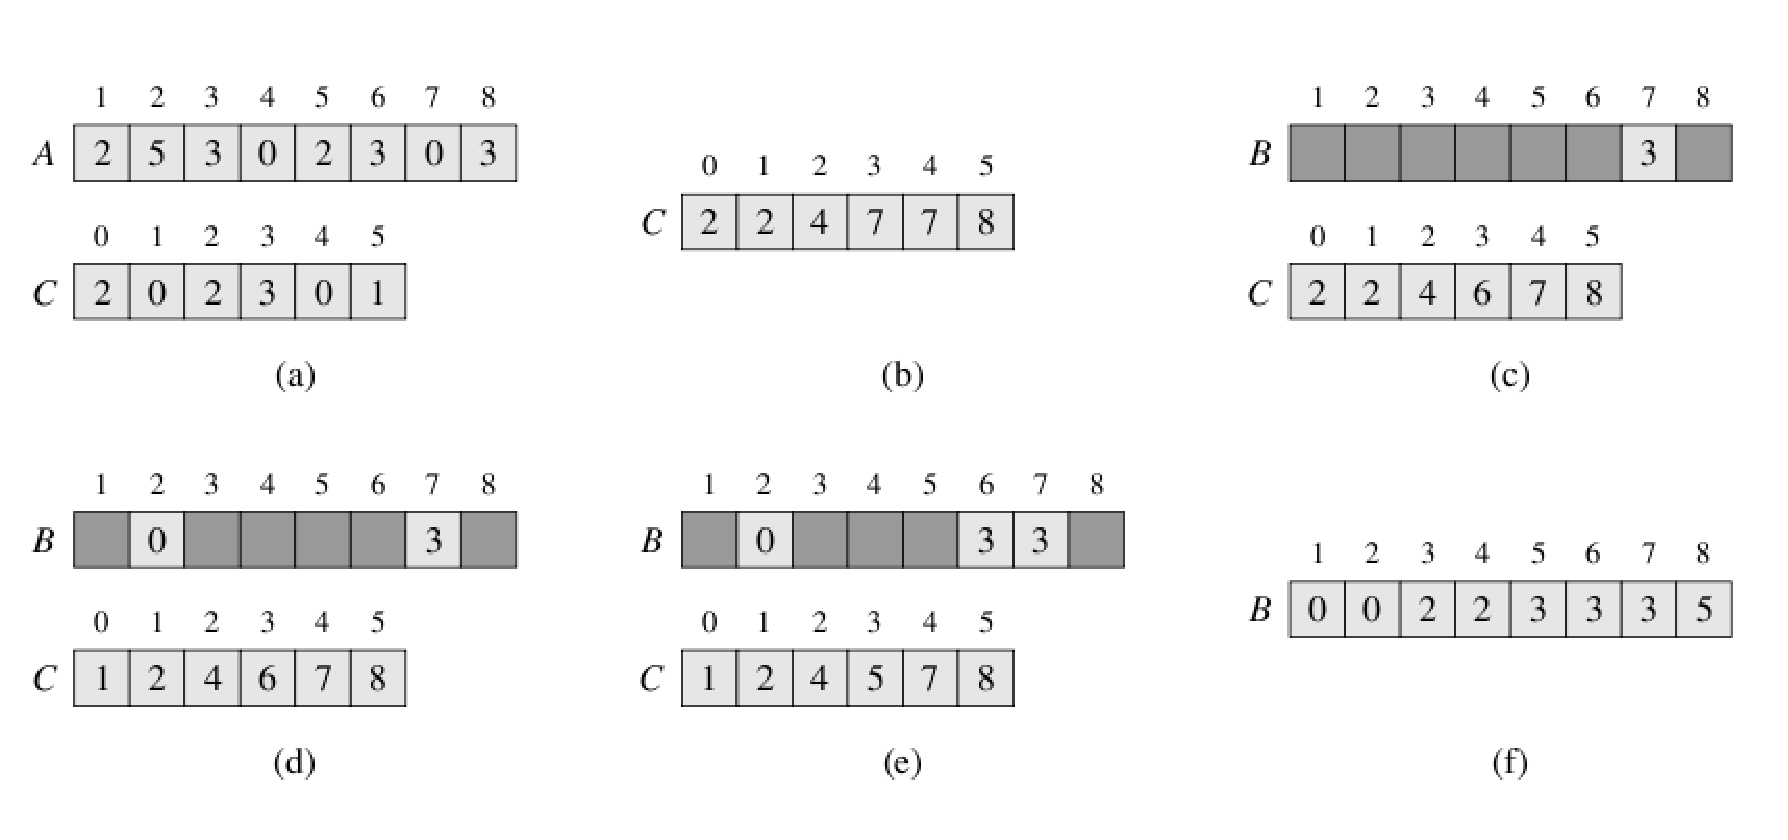
\includegraphics[width=5in]{lecture5/counting-sort.eps}

Анализ: первый и третий циклы требуют $\mathcal{O}(k)$, второй и четвёртый --
$\mathcal{O}(k)$, таким образом время выполнения алгоритма в целом составляет
$\mathcal{O}(n+k)$.

Если $k = \mathcal{O}(n)$, то сортировка подсчётом работает за линейное время!
Однако наша теорема говорила об обратном! Тем не менее всё вышесказанное
правильно, т.к. сортировка подсчётом не использует сравнения.

Важное свойство сортировки подсчётом: стабильность.

Стабильность сортировки означает, что она сохраняет относительный порядок равных
элементов. Это важно к примеру для использования сортировки подсчётом в
поразрядной сортировке.

Упражнение: подумать какие из уже известных нам алгоритмов сортировки являются
стабильными.

\section{Поразрядная сортировка}

\subsection{Идея}
Предложена Германом Холлеритом для переписи населения в США в 1890-м году, т.о.
является чуть ли самой старой имплементацией сортировки.

Сортировались перфокарты (размером 80 на 16). Нужно было отсортировать каждый
столбец.

Первая идея: сортировать карты по первой, самой старшей цифре. Плохая идея, т.к.
после такой сортировки нужно было разбивать всю стопку карт на 10 котейнеров и
продолжать сортировку в них, снова разбивая и т.д. Тяжело поддерживать сразу
много контейнеров.

Хорошая идея: сортировать по младшей цифре, использую стабильную сортировку как
подпрограмму, тогда можно обойтись только одним контейнером.

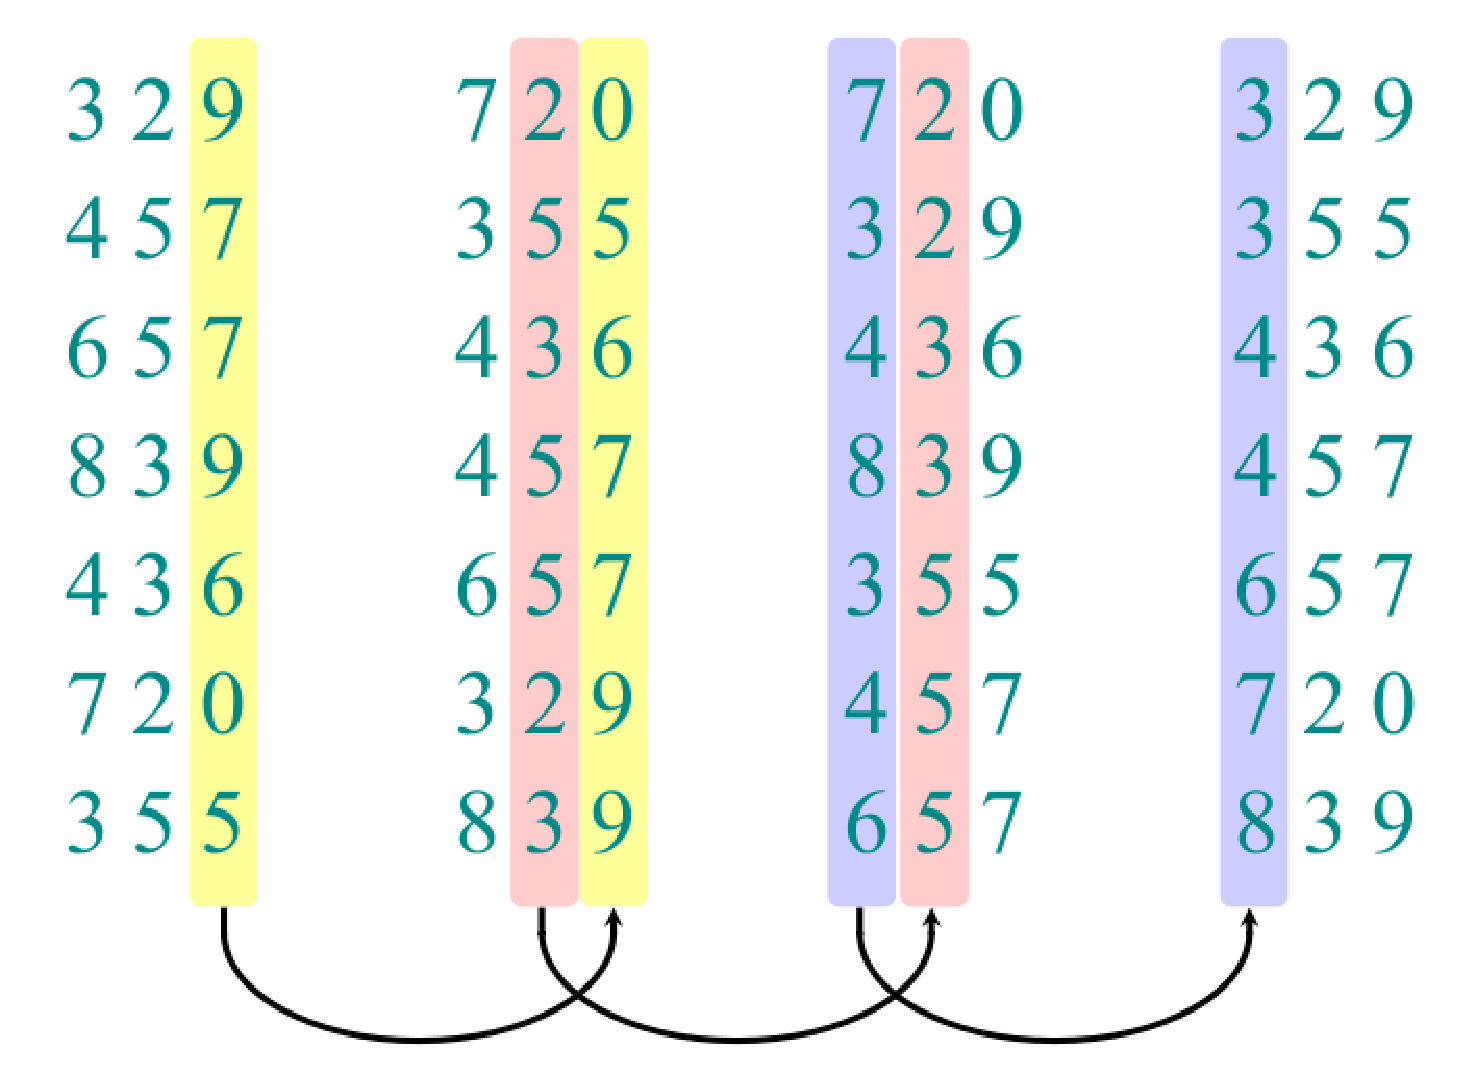
\includegraphics[width=5in]{lecture5/radix-example.eps}

\subsection{Корректность}

Доказательство корректности алгоритма: математическая индукция по позиции цифры
(по колонке).

Гипотеза: Пусть $t-1$ колонок (числа, состоящие из младших $t-1$ цифр) уже
отсортированы и мы сортируем по $t$-й цифре (колонке).

Предположим, что мы сравниваем две цифры в $t$-й колонке. Есть два варианта:

\begin{itemize}
\item Они равны. Тогда поскольку наша вспомогательная сортировка стабильна --
  мы сохраним порядок. А по гипотезе индукции предыдущие цифры уже были
  отсортированы. Потому в итоге получим что наши числа окажутся в правильном
  порядке.
\item Они неравны. Тогда наша сортировка расставит числа в правильном порядке,
  поскольку значение числа определяется его старшей цифрой, которую мы как раз и
  отсортируем в этом шаге.
\end{itemize}

\subsection{Анализ}
Будем использовать в качестве вспомогательной стабильной сортировки --
сортировку подсчётом.

Предположим, что нам нужно отсортировать $n$ чисел, каждое из которых состоит из
$b$ бит.

Плохая идея работать с чисто битовым представлением, т.к. предположим, что наши
числа находятся в диапозоне от $0$ до $n$ и их $n$, тогда двоичное представление
таких чисел будет занимать $\lg n$ и соответственно нам надо будет пройтись по
ним $\lg n$ раз, то есть суммарное время выполнения будет $\mathcal{O}(n \lg
n)$, что хуже линейнего.

Но у нас есть контроль над размером ``цифры''. Можно сгруппировать биты в группы
и назвать их ``цифрами''. Предположим, что мы группируем биты в группы по $r$
бит, таким образом получаем, что наши числа записаны в системе счисления с
основанием $2^r$. Тогда наше число записано с помощью $b/r$ цифр.

Пример: 32-битное слово разбиваем на группы по 8 бит:

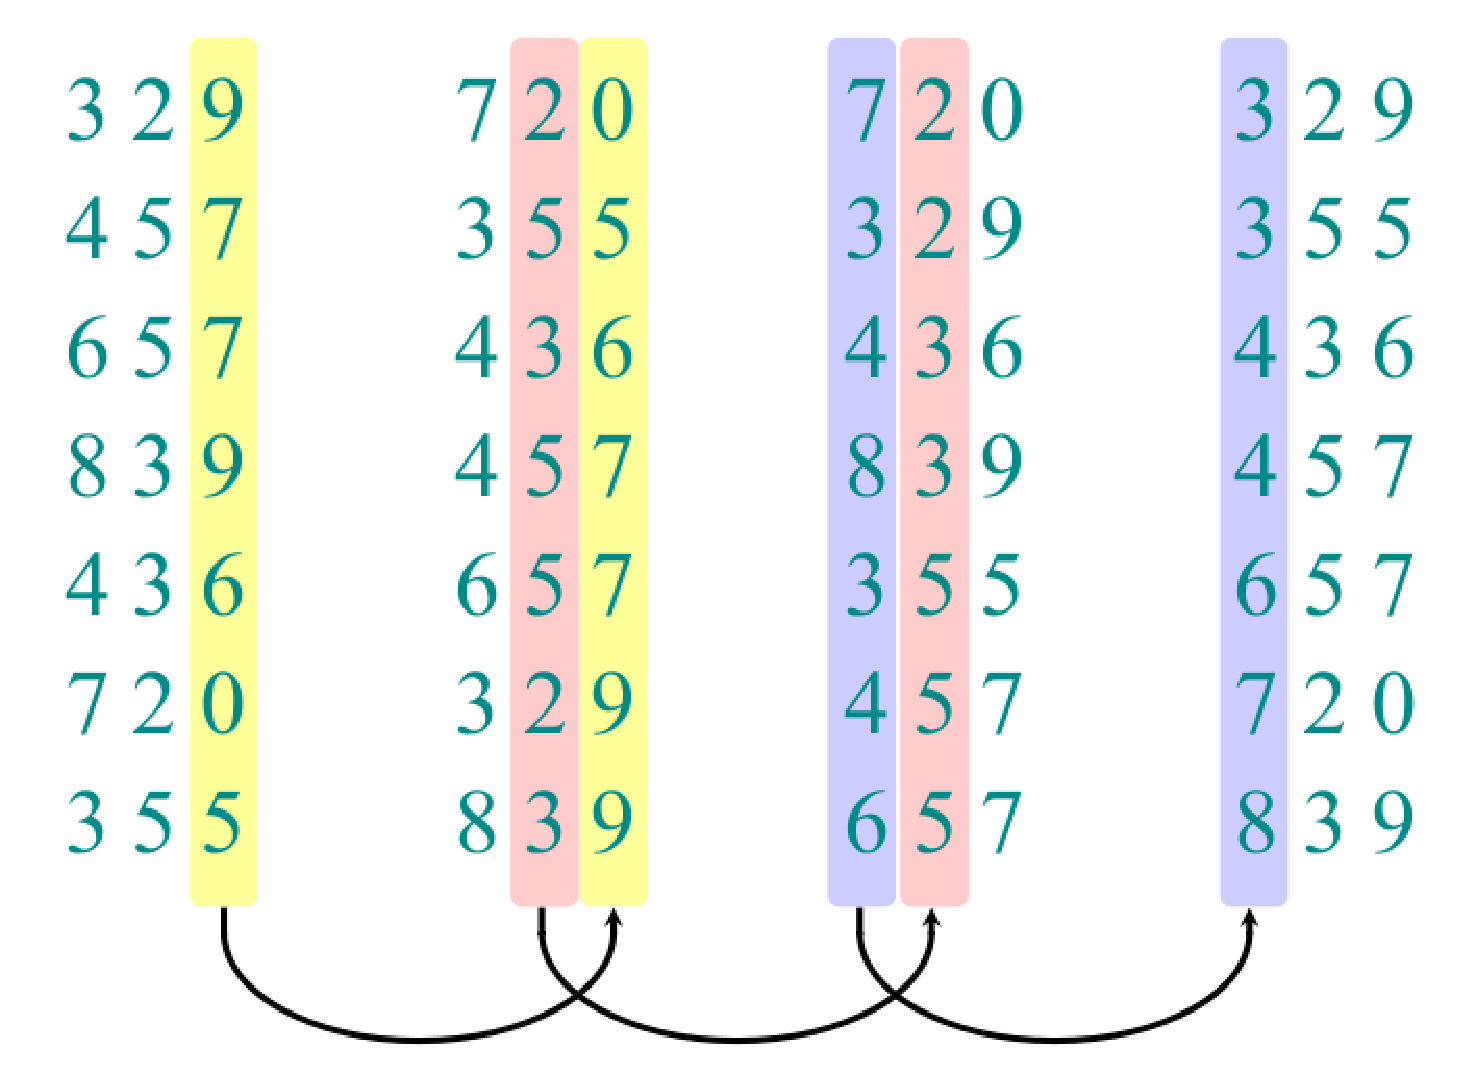
\includegraphics[width=5in]{lecture5/radix-example.eps}

Таким образом здесь $r=8, b/r=4$ прохода по цифрам в системе счисления с базой
$2^8$

Вопрос в том как оптимально разбить биты на группы.

Вспомним, что время сортировка подсчётом $O(n+k)$ для того чтобы отсортировать
числа в диапазоне от 0 до $k-1$. Если мы будем разбивать на группы по $r$, то
максимально возможной цифрой будет $2^r$ и время выполнения сортировки подсчётом
будет $O(n + 2^r)$. Количество проходов алгоритма же равно количеству ``цифр'',
то есть $b/r$. То есть финальная оценка равна $T(n,b) = \Theta((b/r)(n+2^r))$

попробуем минимизировать $T(n,b)$ управляя $r$. Минимум можно найти с помощью
дифферинцирования по $r$, но мы сделаем проще.

Увеличение $r$ означает уменьшение количества проходов, однако в правом
множителе $2^r$ растёт гораздо быстрее.

Мы не хотим, чтобы $2^r >> n$, поэтому мы выбираем $r = \lg n$.

Таким образом получается, что $T(n, b) = \Theta(bn/\lg n)$

Для чисел в диапазоне от 0 до $n^d - 1$ количество бит $b = d \lg n$, потому
время выполнение будет равно $\Theta(dn)$.

\end{document}

